\documentclass{beamer}\usepackage[]{graphicx}\usepackage[]{xcolor}
% maxwidth is the original width if it is less than linewidth
% otherwise use linewidth (to make sure the graphics do not exceed the margin)
\makeatletter
\def\maxwidth{ %
  \ifdim\Gin@nat@width>\linewidth
    \linewidth
  \else
    \Gin@nat@width
  \fi
}
\makeatother

\definecolor{fgcolor}{rgb}{0.345, 0.345, 0.345}
\newcommand{\hlnum}[1]{\textcolor[rgb]{0.686,0.059,0.569}{#1}}%
\newcommand{\hlstr}[1]{\textcolor[rgb]{0.192,0.494,0.8}{#1}}%
\newcommand{\hlcom}[1]{\textcolor[rgb]{0.678,0.584,0.686}{\textit{#1}}}%
\newcommand{\hlopt}[1]{\textcolor[rgb]{0,0,0}{#1}}%
\newcommand{\hlstd}[1]{\textcolor[rgb]{0.345,0.345,0.345}{#1}}%
\newcommand{\hlkwa}[1]{\textcolor[rgb]{0.161,0.373,0.58}{\textbf{#1}}}%
\newcommand{\hlkwb}[1]{\textcolor[rgb]{0.69,0.353,0.396}{#1}}%
\newcommand{\hlkwc}[1]{\textcolor[rgb]{0.333,0.667,0.333}{#1}}%
\newcommand{\hlkwd}[1]{\textcolor[rgb]{0.737,0.353,0.396}{\textbf{#1}}}%
\let\hlipl\hlkwb

\usepackage{framed}
\makeatletter
\newenvironment{kframe}{%
 \def\at@end@of@kframe{}%
 \ifinner\ifhmode%
  \def\at@end@of@kframe{\end{minipage}}%
  \begin{minipage}{\columnwidth}%
 \fi\fi%
 \def\FrameCommand##1{\hskip\@totalleftmargin \hskip-\fboxsep
 \colorbox{shadecolor}{##1}\hskip-\fboxsep
     % There is no \\@totalrightmargin, so:
     \hskip-\linewidth \hskip-\@totalleftmargin \hskip\columnwidth}%
 \MakeFramed {\advance\hsize-\width
   \@totalleftmargin\z@ \linewidth\hsize
   \@setminipage}}%
 {\par\unskip\endMakeFramed%
 \at@end@of@kframe}
\makeatother

\definecolor{shadecolor}{rgb}{.97, .97, .97}
\definecolor{messagecolor}{rgb}{0, 0, 0}
\definecolor{warningcolor}{rgb}{1, 0, 1}
\definecolor{errorcolor}{rgb}{1, 0, 0}
\newenvironment{knitrout}{}{} % an empty environment to be redefined in TeX

\usepackage{alltt}
\usepackage{graphicx}
\usepackage{graphicx}
\usepackage{verbatim}
\usepackage{etoolbox}
\usepackage{everysel}
% \usepackage{enumitem}

%% This package allows text highlighting
\usepackage{soul}

%% This sets the theme of the presentation which controls
%% the formatting of the slides
\usetheme{Boadilla}

%% Turn off the navigation symbols
\setbeamertemplate{navigation symbols}{} 

%% Change the default itemize [ball]s to [circle]s
\setbeamertemplate{itemize items}[circle]

%% Change the default enumerate [ball]s to plain text
\setbeamertemplate{enumerate items}[default]

%% Load the enumitem package and ensure it works nicely with beamer
% \setitemize{label=\usebeamerfont*{itemize item}
%   \usebeamercolor[fg]{itemize item}
%   \usebeamertemplate{itemize item}}
% \setenumerate{label=\usebeamerfont*{enumerate item}
%   \usebeamercolor[fg]{enumerate item}
%   \usebeamertemplate{enumerate item}}

%% Set the author block so STATS 201/8 appears on every
\author{STATS 201/8}

%% Clear the date block
\date{}


\setbeamercolor{title}{bg=blue!40}
\setbeamerfont{title}{size=\LARGE,series=\bfseries}

%%Sectioning commands
\setbeamercolor{section title}{bg=blue!20}
\setbeamerfont{section title}{size=\large}

\setbeamertemplate{section page}{%
    \begingroup
        \begin{beamercolorbox}[sep=10pt,center,rounded=true,shadow=true]{section title}
        \usebeamerfont{section title}Section~\thechapter.\thesection \newline \insertsection\par
        \end{beamercolorbox}
		\vfill
    \endgroup
}

\newcommand{\BeginSection}[1]{\section{#1} \frame{\sectionpage}}
%\AtBeginSection[]{%
%    \begin{frame}
%        \sectionpage
%    \end{frame}
%}


%% This makes all equations blue
\AtBeginEnvironment{equation*}{\color{blue}}
\AtBeginEnvironment{align*}{\color{blue}}
\everymath{\color{blue}}

%% This puts a 0 point space between paragraphs, means we don't need to use vspace, or list environments if 
%% we don't want to
\setlength{\parskip}{0pt}


%% Russell: removes spaces after R input/output?
\setlength{\topsep}{0.5mm}

%% David: In addition to Russel's command to remove spaces after R input/output, these commands remove the space between R input/output.
%% Stackoverflow link: https://stackoverflow.com/questions/35734525/reduce-space-between-code-chunks-and-code-output-in-rmarkdown-beamer-presentatio
%% \setlength{\OuterFrameSep}{-2pt}
\makeatletter
\preto{\@verbatim}{\topsep=-1pt \partopsep=-1pt }
\makeatother

%% Some useful colors
\definecolor{darkgreen}{rgb}{0.176,0.486,0.031}
\definecolor{redbrown}{HTML}{950605}
\definecolor{darkred}{HTML}{d80605}


%% nice little macro for changing the font of R code
\newcommand{\rcode}[1]{\protect{\color{darkgreen}\texttt{#1}}}

%% macro for bold blue italics
\newcommand{\blueBoldEmph}[1]{{\color{blue}\textbf{\emph{#1}}}}

% ~iid macro
\newcommand{\iid }{\stackrel{iid}{\sim}}

%% Macro for t-test amd P-value
\newcommand{\ttest}{\emph{t}-test}
\newcommand{\pval}{\emph{P}-value}

%% Statistics operators 
\DeclareMathOperator{\Bias}{Bias}
\DeclareMathOperator{\Cov}{Cov}
\DeclareMathOperator*{\Cor}{Cor}
\DeclareMathOperator{\E}{E}
\DeclareMathOperator{\MSE}{MSE}
\DeclareMathOperator{\Odds}{Odds}
\DeclareMathOperator{\OR}{OR}
\DeclareMathOperator{\PMSE}{PMSE}
\DeclareMathOperator{\sd}{sd}
\DeclareMathOperator{\se}{se}
\DeclareMathOperator*{\Var}{Var}
\DeclareMathOperator{\logit}{logit}

%% Should see if can make this a mathop
\newcommand{\comb}[2]{\mbox{$\big(_{#2}^{#1}\big)$}}



\IfFileExists{upquote.sty}{\usepackage{upquote}}{}
\begin{document}
\newcommand{\thechapter}{11}



\title{Chapter \thechapter: \\ Linear models with a single factor explanatory variable having three or more levels \\ (One-way analysis of variance)}

\institute{University of Auckland}


\begin{frame}
\titlepage
\end{frame}


\begin{frame}[t]
\frametitle{Learning Outcomes}
In this chapter you will learn about:
\begin{center}
\vspace{16pt}
  \begin{itemize}
  \item Fitting a model with a single explanatory factor variable with multiple levels, a.k.a., one-way analysis of variance (ANOVA)\footnote{{\bf NOTE:} When people use the term ANOVA (Analysis of Variance),
they are referring to a linear regression model in which all the explanatory variable are factors.}
  \item Interpretting the fitted model
  \item Multiple pairwise comparisons of means
  \item Using \rcode{emmeans} to solve the multiple comparisons problem 
  \item Relevant \rcode{R}-code
  \item Alternative parameterizations of the one-way ANOVA model\footnote{Optional section.}
  \end{itemize}
\end{center}

\end{frame}



%%%%%%%%%%%%%%%%%%%%%%%%%%%%%%%%%%%%%%%%%%%%%%%%%%%%%%%%%%%%%%%%%%%%%%%%%%%%%%%%%%%%%%%%%%%
\BeginSection{Example with a 5-level explanatory factor variable }
%%%%%%%%%%%%%%%%%%%%%%%%%%%%%%%%%%%%%%%%%%%%%%%%%%%%%%%%%%%%%%%%%%%%%%%%%%%%%%%%%%%%%%%%%%%


% \begin{frame}
% \begin{center}
% {\huge Explanatory factor with multiple levels, \\
%  and the multi comparisons problem}
% \end{center}
% \end{frame}


\begin{frame}[fragile]
% \frametitle{Explanatory factor with many levels ($>2$)}
% \framesubtitle{Fruit fly example}
\frametitle{Example -- Fruit flies}

In this case study we look at how the male fruit-fly's longevity is related
to his reproductive activity.

\begin{center}
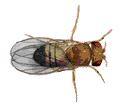
\includegraphics[scale=0.9]{Pictures/rfly}
\end{center}

Fruit flies are a very commonly used animal for laboratory experiments because they are easy to maintain and breed. Their short lifespan allows several generations to be observed within a few months. They also have a genome that is very close to that of humans with many genes discovered in humans also found in fruit flies.\footnote{
See \url{https://www.yourgenome.org/facts/why-use-the-fly-in-research} for more background on research with fruit flies.}
\medskip

Previous studies have shown that the longevity (life span) of female fruit flies decreases with an increase in reproduction, and this leads to a similar question related to males.
\end{frame}


\begin{frame}[fragile]
\frametitle{Fruit fly}
The experiment compared the lifespan of males that were divided into 5 treatment groups that varied according to the presence or absence and number of uninterested or interested females.\footnote{Had there been only two treatment groups then we could have used the two sample two-sample \ttest{} discussed in Chapter 5}
\medskip

How does one define ``interest" in female fruit flies? Here is this study's definition:
\begin{itemize}
\item [] Newly inseminated females will not usually mate again for at least two days.
So, the males in the uninterested females treatment groups were always living
with newly inseminated females.
\end{itemize}
\bigskip

The {\bf primary focus of this Example} is the following: Due to the explanatory factor variable (treatment group) having several levels, we will need to apply an adjustment to relevant \pval{s} and confidence intervals when we are making inference about differences in the expected lifespans between pairs of treatment groups.
\end{frame}



\begin{frame}[fragile]
\frametitle{Fruit fly\ldots}

The response variable measured was \rcode{days}, the number of days the male fly lived.
\bigskip
  

The explanatory factor variable was \rcode{group}, with five levels:

\begin{itemize}
 \item  \rcode{G1} males living alone, \\
 \item  \rcode{G2} males living with one interested female, \\
 \item  \rcode{G3} males living with eight interested females,\\
 \item  \rcode{G4} males living with one uninterested female, and \\
 \item  \rcode{G5} males living with eight uninterested females.
\end{itemize}
\medskip

There were 25 male flies in each group, for a total sample size of 125.
\end{frame}


\begin{frame}[fragile]
\frametitle{Fruit fly\ldots}

Let us take a look at the data:
\begin{knitrout}\scriptsize
\definecolor{shadecolor}{rgb}{0.969, 0.969, 0.969}\color{fgcolor}\begin{kframe}
\begin{alltt}
\hlstd{> }\hlstd{Fruitfly.df} \hlkwb{=} \hlkwd{read.csv}\hlstd{(}\hlstr{"Data/Fruitfly.csv"}\hlstd{,} \hlkwc{header}\hlstd{=T)}
\hlstd{> }\hlstd{Fruitfly.df}\hlopt{$}\hlstd{group}\hlkwb{=}\hlkwd{factor}\hlstd{(Fruitfly.df}\hlopt{$}\hlstd{group)}
\hlstd{> }\hlkwd{boxplot}\hlstd{(days} \hlopt{~} \hlstd{group,} \hlkwc{data} \hlstd{= Fruitfly.df,} \hlkwc{ylab} \hlstd{=} \hlstr{"Longevity (days)"}\hlstd{)}
\end{alltt}
\end{kframe}
\end{knitrout}



\begin{figure}
  \centering
  \includegraphics{figure/RC-H11-002}
\end{figure}

It looks like male fruit flies do not live as long when in the presence of `uninterested' females (\rcode{G5}), especially when there are several of them.
\end{frame}



\begin{frame}[fragile, label={cnrpt_model}]
\frametitle{Fruit fly\ldots}
\framesubtitle{Linear  model with multi-level ($>2$) explanatory factor}

As seen in previous chapters that involved categorical explanatory variables, our model specification uses indicator variables. In this case:

\[\rcode{days}=\beta_0+\beta_{1}\times\rcode{D2} +\beta_{2}\times\rcode{D3} + \beta_{3}\times\rcode{D4}+  \beta_{4}\times\rcode{D5} + \epsilon\]
where, as usual $\epsilon \iid N(0, \sigma^2)$, and

\medskip
\begin{itemize}
\item \rcode{D2} is an indicator variable whereby \rcode{D2}=1 if the fruit fly is in group 2, otherwise it is 0.

\item \rcode{D3} is an indicator variable whereby \rcode{D3}=1 if the fruit fly is in group 3, otherwise it is 0.

\item ... and so on.
\end{itemize}

For example, $\beta_{1}$ and $\beta_{2}$ represent the differences in expected longevity (\rcode{days}) when we compare groups 2 and 3 to group 1 (the baseline).

%Take a look at the design matrix (5 groups of 4 obs each)
%Grp=rep(c("G1","G2","G3","G4","G5"),c(4,4,4,4,4))
%y=rnorm(20,60,10)
%MadeUpDataFrame=data.frame(Grp,y)
%lmFit=lm(y~Grp,data=MadeUpDataFrame)
%model.matrix(~Grp,data=MadeUpDataFrame)
\end{frame}


\begin{frame}[fragile]
\frametitle{Fruit fly\ldots}
\framesubtitle{Assumption checks}

% Let us see how this model works out with the usual assumption checks.
\begin{knitrout}\scriptsize
\definecolor{shadecolor}{rgb}{0.969, 0.969, 0.969}\color{fgcolor}\begin{kframe}
\begin{alltt}
\hlstd{> }\hlstd{Fruitfly.fit} \hlkwb{=} \hlkwd{lm}\hlstd{(days} \hlopt{~} \hlstd{group,} \hlkwc{data} \hlstd{= Fruitfly.df)}
\hlstd{> }\hlkwd{plot}\hlstd{(Fruitfly.fit,} \hlkwc{which}\hlstd{=}\hlnum{1}\hlstd{)}
\end{alltt}
\end{kframe}
\end{knitrout}



\begin{figure}
  \centering
  \includegraphics{figure/RC-H11-004}
\end{figure}

The {\bf EOV} assumption seem to be okay.
\end{frame}


\begin{frame}[fragile]
\frametitle{Fruit fly\ldots}
\framesubtitle{Assumption checks\ldots}

\begin{knitrout}\scriptsize
\definecolor{shadecolor}{rgb}{0.969, 0.969, 0.969}\color{fgcolor}\begin{kframe}
\begin{alltt}
\hlstd{> }\hlkwd{normcheck}\hlstd{(Fruitfly.fit)}
\end{alltt}
\end{kframe}
\end{knitrout}



\begin{figure}
  \centering
  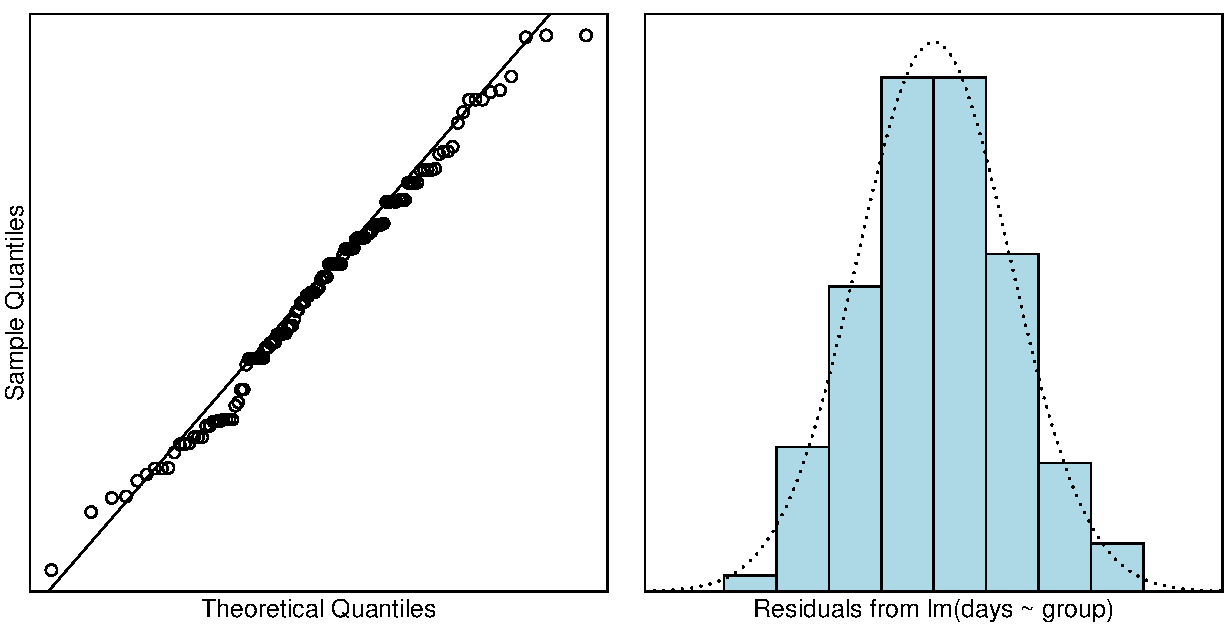
\includegraphics[scale = 0.5]{figure/RC-H11-006}
\end{figure}

The normality assumption seem to be okay.
\end{frame}


\begin{frame}[fragile]

\frametitle{Fruit fly\ldots}
\framesubtitle{Assumption checks\ldots}

\begin{knitrout}\scriptsize
\definecolor{shadecolor}{rgb}{0.969, 0.969, 0.969}\color{fgcolor}\begin{kframe}
\begin{alltt}
\hlstd{> }\hlkwd{cooks20x}\hlstd{(Fruitfly.fit)}
\end{alltt}
\end{kframe}
\end{knitrout}



\begin{figure}
  \centering
  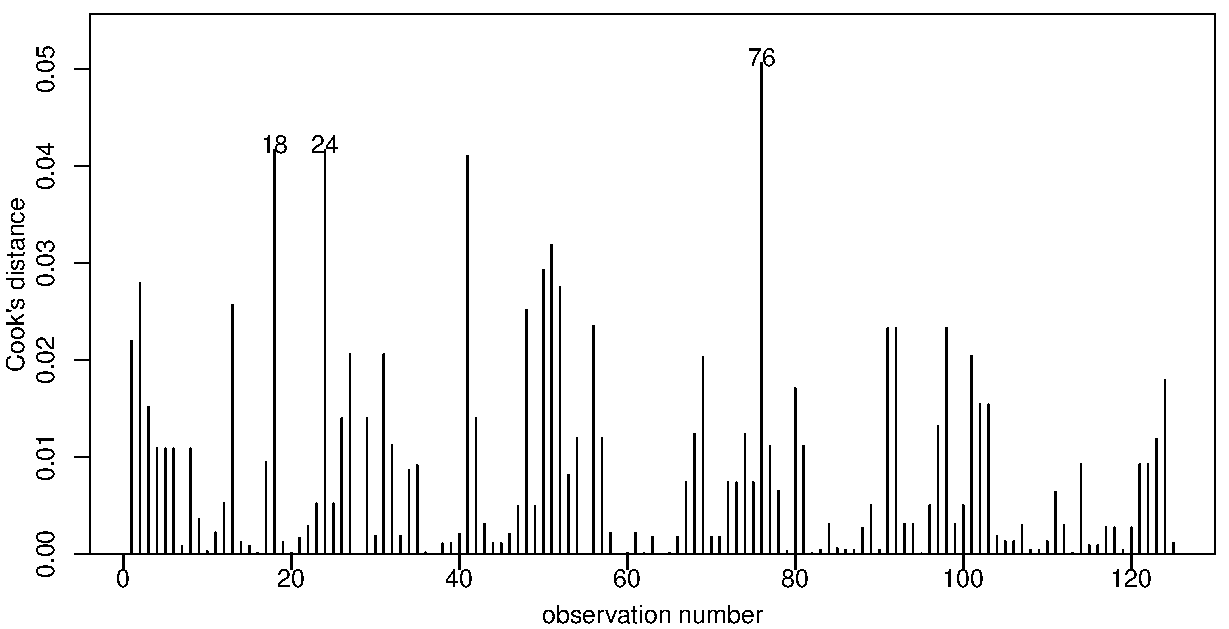
\includegraphics[scale = 0.5]{figure/RC-H11-008}
\end{figure}

No unduly influential data points.

\end{frame}

\begin{frame}[fragile, label={fruitfly_anova}]
\frametitle{Fruit fly\ldots}
\framesubtitle{$R^2$ and ANOVA table}
We can trust the fitted model. What can we conclude?\footnote{Recall from Chapter 9 that we have to use the \rcode{anova} function to check the significance of a factor variable with more than two levels.}
\medskip

\begin{knitrout}\scriptsize
\definecolor{shadecolor}{rgb}{0.969, 0.969, 0.969}\color{fgcolor}\begin{kframe}
\begin{alltt}
\hlstd{> }\hlkwd{anova}\hlstd{(Fruitfly.fit)}
\end{alltt}
\begin{verbatim}
Analysis of Variance Table

Response: days
           Df Sum Sq Mean Sq F value    Pr(>F)    
group       4  11939 2984.82  13.612 3.516e-09 ***
Residuals 120  26314  219.28                      
---
Signif. codes:  0 '***' 0.001 '**' 0.01 '*' 0.05 '.' 0.1 ' ' 1
\end{verbatim}
\end{kframe}
\end{knitrout}

\medskip

This allows us to say that there is very strong evidence of a difference in expected longevity between the five groups, which was fairly obvious from the boxplot.
\smallskip

A significant result means we should now investigate how the groups differ from one another -- there is more work to be done.

\end{frame}


%%%%%%%%%%%%%%%%%%%%%%%%%%%%%%%%%%%%%%%%%%%%%%%%%%%%%%%%%%%%%%%%%%%%%%%%%%%%%%%%%%%%%%%%%%%
\BeginSection{Interpreting the output}
%%%%%%%%%%%%%%%%%%%%%%%%%%%%%%%%%%%%%%%%%%%%%%%%%%%%%%%%%%%%%%%%%%%%%%%%%%%%%%%%%%%%%%%%%%%


\begin{frame}[fragile,label=refcell_coeffs]
\frametitle{Fruit fly\ldots}
\framesubtitle{Interpretation}
Now we know that the variable \rcode{group} helps explain longevity,
what can we say about these groups? Let us investigate.

\begin{knitrout}\scriptsize
\definecolor{shadecolor}{rgb}{0.969, 0.969, 0.969}\color{fgcolor}\begin{kframe}
\begin{alltt}
\hlstd{> }\hlkwd{summary}\hlstd{(Fruitfly.fit)}
\end{alltt}
\end{kframe}
\end{knitrout}

\begin{knitrout}\scriptsize
\definecolor{shadecolor}{rgb}{0.969, 0.969, 0.969}\color{fgcolor}\begin{kframe}
\begin{verbatim}
Coefficients:
            Estimate Std. Error t value Pr(>|t|)    
(Intercept)   63.560      2.962  21.461  < 2e-16 ***
groupG2        1.240      4.188   0.296    0.768    
groupG3       -0.200      4.188  -0.048    0.962    
groupG4       -6.800      4.188  -1.624    0.107    
groupG5      -24.840      4.188  -5.931 2.98e-08 ***
---
Residual standard error: 14.81 on 120 degrees of freedom
Multiple R-squared:  0.3121,	Adjusted R-squared:  0.2892 
F-statistic: 13.61 on 4 and 120 DF,  p-value: 3.516e-09
\end{verbatim}
\end{kframe}
\end{knitrout}

Our fitted model only gives the pairwise difference between the baseline group \rcode{G1} and the other four groups, and so is only providing partial information. What else can we do?
\end{frame}


\begin{frame}[fragile]
\frametitle{Fruit fly\ldots}
\framesubtitle{Interpretation of grand and group means}
Some researchers like to examine the group means and their
deviations from the overall (or so-called``grand'') mean.\footnote{See the optional final Section of this Chapter for more on this topic.} 
These deviations are commonly called group ``effects''.
\medskip

The estimated grand mean is simply the sample mean over all 125 male flies:
\begin{knitrout}\scriptsize
\definecolor{shadecolor}{rgb}{0.969, 0.969, 0.969}\color{fgcolor}\begin{kframe}
\begin{alltt}
\hlstd{> }\hlstd{grand.mean}\hlkwb{=}\hlkwd{mean}\hlstd{(Fruitfly.df}\hlopt{$}\hlstd{days)}
\hlstd{> }\hlstd{grand.mean}
\end{alltt}
\begin{verbatim}
[1] 57.44
\end{verbatim}
\end{kframe}
\end{knitrout}

The estimated group means are just the sample means within each group. We can quickly obtain these using the incredibly useful\footnote{\rcode{dplyr} and its associated packages are widely used for ``data wrangling'' (the process of cleaning and re-arranging data sets for easy access and analysis).} \rcode{dplyr} package:


\begin{knitrout}\scriptsize
\definecolor{shadecolor}{rgb}{0.969, 0.969, 0.969}\color{fgcolor}\begin{kframe}
\begin{alltt}
\hlstd{> }\hlkwd{library}\hlstd{(}\hlkwd{dplyr}\hlstd{())}
\hlstd{> }\hlstd{Df}\hlkwb{=}\hlstd{Fruitfly.df} \hlopt \hlkwd{group_by}\hlstd{(group)} \hlopt \hlkwd{summarize}\hlstd{(}\hlkwc{group.mean}\hlstd{=}\hlkwd{mean}\hlstd{(days))} \hlopt
\hlstd{+ }  \hlkwd{data.frame}\hlstd{()}
\end{alltt}
\end{kframe}
\end{knitrout}

\end{frame}



\begin{frame}[fragile, label={group_means}]
\frametitle{Fruit fly\ldots}
\framesubtitle{Interpretation of grand and group means}
The above code groups the data by \rcode{group} and then applies the \rcode{mean} function to the \rcode{days} values within each group.
\medskip

The estimated group means are
\begin{knitrout}\scriptsize
\definecolor{shadecolor}{rgb}{0.969, 0.969, 0.969}\color{fgcolor}\begin{kframe}
\begin{alltt}
\hlstd{> }\hlstd{Df}\hlopt{$}\hlstd{group.mean}
\end{alltt}
\begin{verbatim}
[1] 63.56 64.80 63.36 56.76 38.72
\end{verbatim}
\end{kframe}
\end{knitrout}
and the estimated group effects are therefore
\begin{knitrout}\scriptsize
\definecolor{shadecolor}{rgb}{0.969, 0.969, 0.969}\color{fgcolor}\begin{kframe}
\begin{alltt}
\hlstd{> }\hlstd{Df}\hlopt{$}\hlstd{group.mean}\hlopt{-}\hlstd{grand.mean}
\end{alltt}
\begin{verbatim}
[1]   6.12   7.36   5.92  -0.68 -18.72
\end{verbatim}
\end{kframe}
\end{knitrout}
\medskip

We have seen that the overall average longevity of the 125 male flies in the study
is about 57.4 days.
\medskip 

We also see that group \rcode{G5} has markedly lower longevity (18.72 fewer days) compared to the overall mean.
\bigskip

We could test null hypotheses and calculate confidence intervals for the above conclusions, but our focus on this course will be making inference about the differences in group means.
\end{frame}



\begin{frame}[fragile]
\frametitle{Fruit fly\ldots}
\framesubtitle{Pairwise comparisons}
We'd really like to get the pairwise comparisons between every possible pair of groups.
However, we've seen that the fitted model is restricted to examining how the groups \rcode{G2-G5} differ from  the baseline group \rcode{G1}.
\medskip

If we wish to see how the other groups differed from group \rcode{G2}, say, then we could achieve this by changing the baseline group to group \rcode{G2}. Recall that this can be done using the \rcode{relevel} function:

\begin{knitrout}\scriptsize
\definecolor{shadecolor}{rgb}{0.969, 0.969, 0.969}\color{fgcolor}\begin{kframe}
\begin{alltt}
\hlstd{> }\hlstd{Fruitfly.df}\hlopt{$}\hlstd{newgroup} \hlkwb{=} \hlkwd{relevel}\hlstd{(Fruitfly.df}\hlopt{$}\hlstd{group,} \hlkwc{ref}\hlstd{=}\hlstr{"G2"}\hlstd{)}
\end{alltt}
\end{kframe}
\end{knitrout}

But to get all pairwise comparisons (i.e., \rcode{G3~vs~G4}, \rcode{G4~vs~G5}, \rcode{\ldots}) we have to do this re-leveling for \rcode{G2}, \rcode{G3} and \rcode{G4}, and refit the model each time. This is too tedious.
\medskip

We can get \rcode{R} to do the `heavy lifting' for us by using the \rcode{emmeans} function from the \rcode{R} package of the same name. Moreover, \rcode{emmeans} solves the multiple comparisons problem that is discussed below.

\end{frame}



%%%%%%%%%%%%%%%%%%%%%%%%%%%%%%%%%%%%%%%%%%%%%%%%%%%%%%%%%%%%%%%%%%%%%%%%%%%%%%%%%%%%%%%%%%%
\BeginSection{The multiple comparisons problem}
%%%%%%%%%%%%%%%%%%%%%%%%%%%%%%%%%%%%%%%%%%%%%%%%%%%%%%%%%%%%%%%%%%%%%%%%%%%%%%%%%%%%%%%%%%%


\begin{frame}[fragile]
\frametitle{Fruit fly\ldots}
\framesubtitle{Multiple comparisons}

Note that when we are looking at all pair-wise comparisons of 5 groups,
we have a total of 10 different possibilities: \medskip

\rcode{G1~vs~G2}, \rcode{G1~vs~G3}, \rcode{G1~vs~G4}, \rcode{G1~vs~G5}, (4 comparisons)

\rcode{G2~vs~G3}, \rcode{G2~vs~G4}, \rcode{G2~vs~G5}, (3 comparisons)

\rcode{G3~vs~G4}, \rcode{G3~vs~G5}, (2 comparisons)

\rcode{G4~vs~G5}, (1 comparisons).

\medskip
In general, if there are $m$ groups then there are $^{m}C_2$ possible pairwise comparisons.\footnote{In \rcode{R} this is given by \rcode{choose(m,2)} and is the number of ways of choosing 2 objects from $m$ objects. E.g., \rcode{choose(5,2)=10}.}

\medskip
Each comparison requires a hypothesis test for a significant difference and an accompanying confidence interval. The multiple comparisons problem arises because, of all null hypotheses that are true, 5\% are falsely rejected (Type 1 error). Equivalently, of all 95\% confidence intervals, 5\% of them do not contain the true parameter value.

\end{frame}



\begin{frame}[fragile]
\frametitle{Erroneous evidence of an effect from multiple testing}
\framesubtitle{Multiple comparisons\ldots}
The following \rcode{R} code fits a simple linear regression model to iid (independent and identically distributed) normal data.  

\medskip

{\bf NOTE:} The null hypothesis $H_0:$ slope = 0 is {\bf true}. 

\begin{knitrout}\scriptsize
\definecolor{shadecolor}{rgb}{0.969, 0.969, 0.969}\color{fgcolor}\begin{kframe}
\begin{alltt}
\hlstd{> }\hlstd{x} \hlkwb{=} \hlnum{1}\hlopt{:}\hlnum{30} \hlcom{## Our explanatory variable}
\hlstd{> }\hlstd{x}
\end{alltt}
\begin{verbatim}
 [1]  1  2  3  4  5  6  7  8  9 10 11 12 13 14 15 16 17 18 19 20 21 22 23 24 25
[26] 26 27 28 29 30
\end{verbatim}
\begin{alltt}
\hlstd{> }\hlstd{y} \hlkwb{=} \hlkwd{rnorm}\hlstd{(}\hlnum{30}\hlstd{)} \hlcom{## y has NO relationship with x}
\hlstd{> }\hlkwd{summary}\hlstd{(}\hlkwd{lm}\hlstd{(y}\hlopt{~}\hlstd{x))}\hlopt{$}\hlstd{coef} \hlcom{## Print only the coefficient table}
\end{alltt}
\begin{verbatim}
              Estimate Std. Error   t value   Pr(>|t|)
(Intercept)  0.4945317  0.3884378  1.273130 0.21344114
x           -0.0413633  0.0218802 -1.890444 0.06908972
\end{verbatim}
\end{kframe}
\end{knitrout}

If this code is run many times over, then approximately 5\% of the time the slope will have \pval{} $<0.05$.\footnote{In fact, it can be shown that the \pval{} is uniformly distributed between 0 and 1 when $H_0$ is true.} \\
\smallskip
That is, there will be erroneous evidence of an effect of \rcode{x} (i.e., evidence for a non-zero slope) about 1 time in 20!

\end{frame}


\begin{frame}[fragile]
\frametitle{Erroneous evidence of an effect from multiple testing\ldots}
\framesubtitle{Multiple comparisons\ldots}

When we do multiple tests (i.e., the 10 paired comparisons in this example) then we greatly increase the probability of obtaining at least one erroneous conclusion\footnote{ Assuming independent comparisons, if we do 10 95\% CIs we have an overall error rate of $1-(1-.05)^{10}=40\%$, which is much higher than our original 5\% error rate per comparison.}.

\medskip 

This is known as the multiple comparison problem. It essentially says that if you look at enough things you will find something `happening', even when there's nothing going on.

\medskip

Remember, data always have variability, and if we are not careful we can `discover' false structure that is not really there.

\medskip 

So, when we look at these 10 comparisons we need to adjust so that the overall error rate (the probability of any spurious significance) over all 10 comparison is no more the 5\%. This can be done using a Tukey adjustment.

\end{frame}


\begin{frame}[fragile]
\frametitle{Example---Fruit fly}
\framesubtitle{Tukey simultaneous confidence intervals}
% \framesubtitle{Multiple comparisons\ldots}

Let's get {\em simultaneous} 95\% confidence intervals for all 10 comparisons via the \rcode{pairs} and \rcode{emmeans} functions of the \rcode{emmeans} package.\footnote{These confidence intervals are called ``simultaneous'' since we can be 95\% confident that {\bf they all} contain the true group difference simultaneously.}

%<<RC-H11-015, size = "scriptsize",warning=F>>=
%library(emmeans)
%Fruitfly.emm = emmeans(Fruitfly.fit, specs = pairwise~group, infer=T)
%Fruitfly.emm$contrasts
%@

\begin{knitrout}\scriptsize
\definecolor{shadecolor}{rgb}{0.969, 0.969, 0.969}\color{fgcolor}\begin{kframe}
\begin{alltt}
\hlstd{> }\hlkwd{library}\hlstd{(emmeans)}
\hlstd{> }\hlstd{Fruitfly.pairs} \hlkwb{=} \hlkwd{pairs}\hlstd{(}\hlkwd{emmeans}\hlstd{(Fruitfly.fit,} \hlopt{~}\hlstd{group,} \hlkwc{infer}\hlstd{=T))}
\hlstd{> }\hlstd{Fruitfly.pairs}
\end{alltt}
\begin{verbatim}
 contrast estimate   SE  df t.ratio p.value
 G1 - G2     -1.24 4.19 120  -0.296  0.9983
 G1 - G3      0.20 4.19 120   0.048  1.0000
 G1 - G4      6.80 4.19 120   1.624  0.4854
 G1 - G5     24.84 4.19 120   5.931  <.0001
 G2 - G3      1.44 4.19 120   0.344  0.9970
 G2 - G4      8.04 4.19 120   1.920  0.3127
 G2 - G5     26.08 4.19 120   6.227  <.0001
 G3 - G4      6.60 4.19 120   1.576  0.5158
 G3 - G5     24.64 4.19 120   5.883  <.0001
 G4 - G5     18.04 4.19 120   4.307  0.0003

P value adjustment: tukey method for comparing a family of 5 estimates 
\end{verbatim}
\end{kframe}
\end{knitrout}
\end{frame}


\begin{frame}[fragile]
\frametitle{Fruit fly}
\framesubtitle{Tukey simultaneous confidence intervals\ldots}

We see that the majority of these pairwise comparisons are not significantly different. Let's extract only the CIs where the Tukey adjusted \pval{}s are less than 0.05.

\medskip
  
\begin{knitrout}\scriptsize
\definecolor{shadecolor}{rgb}{0.969, 0.969, 0.969}\color{fgcolor}\begin{kframe}
\begin{alltt}
\hlstd{> }  \hlstd{Fruitfly.pairs}\hlkwb{=}\hlkwd{data.frame}\hlstd{(Fruitfly.pairs)}
\hlstd{> }  \hlcom{## Which pairwise comparisons have a P-value less than 0.05?}
\hlstd{> }  \hlstd{mc.signif} \hlkwb{=} \hlstd{Fruitfly.pairs[,}\hlstr{"p.value"}\hlstd{]} \hlopt{<} \hlnum{0.05}
\hlstd{> }  \hlstd{mc.signif}
\end{alltt}
\begin{verbatim}
 [1] FALSE FALSE FALSE  TRUE FALSE FALSE  TRUE FALSE  TRUE  TRUE
\end{verbatim}
\begin{alltt}
\hlstd{> }  \hlcom{## Print comparisons which have a P-value less than 0.05}
\hlstd{> }  \hlkwd{print}\hlstd{(Fruitfly.pairs[mc.signif, ],} \hlkwc{digits} \hlstd{=} \hlnum{4}\hlstd{)}
\end{alltt}
\begin{verbatim}
   contrast estimate    SE  df t.ratio   p.value
4   G1 - G5    24.84 4.188 120   5.931 2.958e-07
7   G2 - G5    26.08 4.188 120   6.227 7.232e-08
9   G3 - G5    24.64 4.188 120   5.883 3.701e-07
10  G4 - G5    18.04 4.188 120   4.307 3.240e-04
\end{verbatim}
\end{kframe}
\end{knitrout}

{\bf Note} the use of the \rcode{data.frame} function in the above code. We needed to convert \rcode{Fruitfly.pairs} to a dataframe before we could take the subset of rows, otherwise \rcode{emmeans} gets confused and thinks we are doing a smaller number of pairwise comparisons. 

\end{frame}
  

\begin{frame}[fragile]
\frametitle{Fruit fly\ldots}
% \framesubtitle{Tukey simultaneous confidence intervals\ldots}

Some conclusions:
\begin{itemize}
  \item Our model explains 31\% of variability in fruit fly longevity.

  \item We see that group 5 (males with 8 uninterested females) is different from all the others. 

\end{itemize}

On average, group 5 males live fewer days than:

\begin{itemize}

\item Group 1 (males living alone) by 13 to 36 fewer days.

\item Group 2 (males living with one interested female) by 14 to 38 fewer days.

\item Group 3 (males living with eight interested females) by 13 to 36 fewer days.

\item Group 4 (males living with one uninterested female) by 6 to 30 fewer days.
\end{itemize}

\end{frame}


\begin{frame}[fragile]
\frametitle{Fruit fly\ldots}

On a lighter note there is little evidence of a difference in longevity
if no females or only one uninterested female is about,
or if females are there and 'interested' in them ---
but in the presence of multiple uninterested females they die earlier
(they 'drop like flies').

\medskip

Recall also that in the other studies it was seen that females did not live as long if
they reproduced, which can be attributed to the physical demands of producing and laying eggs. With males, perhaps it is sexual frustration that is killing them!

\medskip

For more on this topic see the research article written by Branco et al. (2017, Reproductive activity triggers accelerated male mortality and decreases lifespan: genetic and gene expression determinants in Drosophila. Heredity 118, 221-228 https://doi.org/10.1038/hdy.2016.89) at
\url{https://www.nature.com/articles/hdy201689}.
\end{frame}



%%%%%%%%%%%%%%%%%%%%%%%%%%%%%%%%%%%%%%%%%%%%%%%%%%%%%%%%%%%%%%%%%%%%%%%%%%%%%%%%%%%%%%%%%%%
\BeginSection{Closing remarks and relevant \rcode{R}-code}
%%%%%%%%%%%%%%%%%%%%%%%%%%%%%%%%%%%%%%%%%%%%%%%%%%%%%%%%%%%%%%%%%%%%%%%%%%%%%%%%%%%%%%%%%%%

\begin{frame}[fragile]
\frametitle{Understanding the \rcode{anova} function output}

\begin{knitrout}\scriptsize
\definecolor{shadecolor}{rgb}{0.969, 0.969, 0.969}\color{fgcolor}\begin{kframe}
\begin{alltt}
\hlstd{> }\hlkwd{anova}\hlstd{(Fruitfly.fit)}
\end{alltt}
\begin{verbatim}
Analysis of Variance Table

Response: days
           Df Sum Sq Mean Sq F value    Pr(>F)    
group       4  11939 2984.82  13.612 3.516e-09 ***
Residuals 120  26314  219.28                      
---
Signif. codes:  0 '***' 0.001 '**' 0.01 '*' 0.05 '.' 0.1 ' ' 1
\end{verbatim}
\end{kframe}
\end{knitrout}

In the above output we see that the variability we observe in our longevity data can be broken down into two components \rcode{group} and \rcode{residual}.
\medskip

The amount of variability that the variable \rcode{group} (as shown in the \rcode{Sum Sq} column) explains is $11939$.  
The residual variability (left over) is $26314$. 
The total variability is $11939+26314=38253$. 
The \% of variability explained by \rcode{group} is therefore
{\scriptsize
\[
100\times \left(\frac{11939}{11939+26314}\right) =100\times \left(1-\frac{26314}{11939+26314}\right)=31 \%.
\] }

Note that we have just calculated the $R^2$ -- the proportion of the variability in the response variable that is explained by the explanatory variables, 0.31.

\end{frame}



\begin{frame}[fragile]
\frametitle{Most of the \rcode{R}-code you need for this chapter}

Use box plots to inspect the data for each level of the factor.

\begin{knitrout}\scriptsize
\definecolor{shadecolor}{rgb}{0.969, 0.969, 0.969}\color{fgcolor}\begin{kframe}
\begin{alltt}
\hlstd{> }\hlkwd{boxplot}\hlstd{(days} \hlopt{~} \hlstd{group,} \hlkwc{data} \hlstd{= Fruitfly.df)}
\end{alltt}
\end{kframe}
\end{knitrout}
\medskip

You do not need to create indicator variables - \rcode{R} does that for you.
The baseline can be changed if you wish by using the \rcode{relevel} function.

\begin{knitrout}\scriptsize
\definecolor{shadecolor}{rgb}{0.969, 0.969, 0.969}\color{fgcolor}\begin{kframe}
\begin{alltt}
\hlstd{> }\hlstd{Fruitfly.df}\hlopt{$}\hlstd{newgroup} \hlkwb{=} \hlkwd{relevel}\hlstd{(Fruitfly.df}\hlopt{$}\hlstd{group,} \hlkwc{ref}\hlstd{=}\hlstr{"G2"}\hlstd{)}
\end{alltt}
\end{kframe}
\end{knitrout}

Fit the model and use the ANOVA table to see if any of the means differ from one another (regardless of the baseline chosen).

\begin{knitrout}\scriptsize
\definecolor{shadecolor}{rgb}{0.969, 0.969, 0.969}\color{fgcolor}\begin{kframe}
\begin{alltt}
\hlstd{> }\hlkwd{anova}\hlstd{(Fruitfly.fit)}
\end{alltt}
\end{kframe}
\end{knitrout}

Adjust confidence intervals for multiple pairwise comparisons by using the Tukey adjustment to obtain simultaneous intervals CIs:

\begin{knitrout}\scriptsize
\definecolor{shadecolor}{rgb}{0.969, 0.969, 0.969}\color{fgcolor}\begin{kframe}
\begin{alltt}
\hlstd{> }\hlstd{Fruitfly.pairs} \hlkwb{=} \hlkwd{pairs}\hlstd{(}\hlkwd{emmeans}\hlstd{(Fruitfly.fit,} \hlopt{~}\hlstd{group,} \hlkwc{infer}\hlstd{=T))}
\end{alltt}
\end{kframe}
\end{knitrout}

\end{frame}



%%%%%%%%%%%%%%%%%%%%%%%%%%%%%%%%%%%%%%%%%%%%%%%%%%%%%%%%%%%%%%%%%%%%%%%%%%%%%%%%%%%%%%%%%%%
\BeginSection{Alternative parameterizations of the 1-way ANOVA model \\ ~ \\ 
(This is an optional Section: \\ - your lecturer will advise whether it is examinable)}
%%%%%%%%%%%%%%%%%%%%%%%%%%%%%%%%%%%%%%%%%%%%%%%%%%%%%%%%%%%%%%%%%%%%%%%%%%%%%%%%%%%%%%%%%%%


\begin{frame}[fragile]
\frametitle{Alternative parameterizations of the 1-way ANOVA model}
\framesubtitle{The reference cell model}
  
Recall the linear model\footnote{See slide~\ref{cnrpt_model}.} we used to represent the longevity, in days, of a male fruitfly, i.e.
  
\vspace{-2mm}
  
\[\rcode{days}=\beta_0+\beta_{1}\times\rcode{D2} +\beta_{2}\times\rcode{D3} + \beta_{3}\times\rcode{D4}+  \beta_{4}\times\rcode{D5} + \epsilon\]
  
\vspace{-5mm}
  
The {\em parameters} $\beta_0,\beta_1,\ldots,\beta_4$ denote the true values of some attribute (e.g. longevity) of the population of male fruitflies. Here, $\beta_0$ represents the mean longevity of male fruitflies in group \rcode{G1}. The parameters $\beta_1,\ldots,\beta_4$ represent the deviations in mean longevity of males in groups \rcode{G2,\ldots,G5}, respectively, from the mean longevity of males in group \rcode{G1}. 
  
\medskip
  
The values in the \rcode{Estimate} column of the regression summary table\footnote{See slide~\ref{refcell_coeffs}; Coefficients rounded to 2 decimal places.} result in the following equation for predicted longevity:
    

    
\medskip
  
\begin{center}
\small
$ \widehat{\rcode{days}}=63.56+1.24\times \rcode{D2} + (-0.20)\times \rcode{D3} + (-6.80)\times \rcode{D4} + (-24.84)\times \rcode{D5}$
\end{center}
  
\end{frame}
  

\begin{frame}[fragile]
\frametitle{Alternative parameterizations of the linear model}
\framesubtitle{The reference cell model}
  
\small

Each cell within a column in the table below corresponds to a level of the \rcode{Group} factor. One way to `parametrise' these cells is to use means, i.e. $\mu_1,\mu_2,\ldots,\mu_5$. Another is to select one of the cells as a reference cell (here \rcode{Group G1}) and the remaining cells are then parametrised the deviations of the current row's group mean from the reference cell's group mean.
  
\medskip

\begin{center}
\footnotesize
\renewcommand{\arraystretch}{1.15}
   \begin{tabular}{ccccccrr}
      \hline
      &&& \multicolumn{5}{c}{parameterization} \\
      \cline{4-8}
      Group & Data && Means & Estimate\footnote{See estimates of \rcode{Group} means on slide~\ref{group_means}} &&
         Reference cell & Estimate\footnote{See regression coefficients table on slide\ref{refcell_coeffs}} \\
      \hline
      \rcode{G1} & $40,37,\ldots,44$ && $\mu_1$ & 63.56 && $\beta_0 = \mu_1$ & 63.56 \\
      \rcode{G2} & $46,42,\ldots,92$ && $\mu_2$ & 64.80 && $\beta_1 = \mu_2 - \mu_1$ & 1.24 \\
      \rcode{G3} & $35,37,\ldots,77$ && $\mu_3$ & 63.36 && $\beta_2 = \mu_3 - \mu_1$ & $-0.20$  \\
      \rcode{G4} & $21,40,\ldots,68$ && $\mu_4$ & 56.76 && $\beta_3 = \mu_4 - \mu_1$ & $-6.80$ \\
      \rcode{G5} & $16,19,\ldots,44$ && $\mu_5$ & 38.72 && $\beta_4 = \mu_5 - \mu_1$ & $-24.84$  \\
      \hline
   \end{tabular}
\end{center}

\medskip

The parameterization of the model shown on the previous slide is therefore known as the {\em reference cell} model. 

\end{frame}
  

\begin{frame}[fragile]
\frametitle{Alternative parameterizations of the linear model}
\framesubtitle{The means model}
  
From the above table we can see that there is an alternative, but equivalent, {\em means} model parameterization, i.e. linear model for the longevity of the $j$th ($j=1,2,\ldots,25$) male fruitfly in \rcode{Group} $i$ ($i=1,2,\ldots,5$) may be written as

\medskip

\[ days_{ij} = \mu_i + \epsilon_{ij} \]

where $\mu_i$ denotes the mean longevity, in days, of a male in \rcode{Group} $i$ and, as usual, $\epsilon_{ij} \iid N(0, \sigma^2)$.

\end{frame}


\begin{frame}[fragile]
\frametitle{Alternative parameterizations of the linear model}
\framesubtitle{The effects model}

\small

Another parameterization is to set the overall mean longevity, $\mu$, as the reference and then define the {\em effect}, $\tau_i$, on longevity due to being in \rcode{Group} $i$ as the difference between the  \rcode{Group} $i$ mean and the overall mean, i.e. $ \tau_i = \mu_i - \mu $.

\medskip

\begin{center}
\footnotesize
\renewcommand{\arraystretch}{1.15}
   \begin{tabular}{ccccccrr}
      \hline
      &&& \multicolumn{5}{c}{parameterization} \\
      \cline{4-8}
      Group & Data && Means & Estimate &&
         Effects & Estimate\footnote{See overall mean (57.44 days) and deviations of group means from overall means on slide~\ref{group_means}.} \\
      \hline
      \rcode{G1} & $40,37,\ldots,44$ && $\mu_1$ & 63.56 && $\tau_1 = \mu_1 - \mu$ & 6.12 \\
      \rcode{G2} & $46,42,\ldots,92$ && $\mu_2$ & 64.80 && $\tau_2 = \mu_2 - \mu$ & 7.36 \\
      \rcode{G3} & $35,37,\ldots,77$ && $\mu_3$ & 63.36 && $\tau_3 = \mu_3 - \mu$ & 5.92  \\
      \rcode{G4} & $21,40,\ldots,68$ && $\mu_4$ & 56.76 && $\tau_4 = \mu_4 - \mu$ & $-0.68$ \\
      \rcode{G5} & $16,19,\ldots,44$ && $\mu_5$ & 38.72 && $\tau_5 = \mu_5 - \mu$ & $-18.72$  \\
      \hline
   \end{tabular}
\end{center}

\medskip
  
The linear {\em effects} model for the longevity of the $j$th ($j=1,2,\ldots,25$) male fruitfly in \rcode{Group} $i$ ($i=1,2,\ldots,5$) may therefore be written as

\vspace{-4mm}

\[ days_{ij} = \mu + \tau_i + \epsilon_{ij} \]

\vspace{-5mm}

where, again, $\epsilon_{ij} \iid N(0, \sigma^2)$.

\end{frame}
  

\end{document}
